\documentclass[11pt,oneside]{book}

\usepackage[margin=1in]{geometry}
\usepackage[T1]{fontenc}
\usepackage[utf8]{inputenc}
\usepackage{lmodern}
\usepackage{microtype}
\usepackage{amsmath,amssymb,amsthm,mathtools,bm}
\usepackage{booktabs,array,tabularx}
\usepackage{enumitem}
\usepackage{float}
\usepackage{caption}
\usepackage{xcolor}
\usepackage{hyperref}
\usepackage[most]{tcolorbox}
\usepackage{tikz}
\usepackage{tikz-3dplot}
\usepackage{pgfplots}
\usepackage{fancyhdr}
\usepackage{titlesec}

\pgfplotsset{compat=1.18}
\usetikzlibrary{arrows.meta,calc,positioning,decorations.pathreplacing,patterns,backgrounds,fit,intersections,shadings,decorations.markings}

\definecolor{chapterblue}{HTML}{1F5AA6}
\definecolor{chapterteal}{HTML}{168A8F}
\definecolor{chapterorange}{HTML}{D9822B}
\definecolor{chaptergreen}{HTML}{2D8A4E}
\definecolor{chapterpurple}{HTML}{6B4EAA}
\definecolor{chapterred}{HTML}{B23B3B}
\definecolor{softblue}{HTML}{EAF3FF}
\definecolor{softgreen}{HTML}{EAF8EF}
\definecolor{softorange}{HTML}{FFF4E6}
\definecolor{softpurple}{HTML}{F3EEFF}
\definecolor{softred}{HTML}{FFF0F0}
\definecolor{softgray}{HTML}{F6F7F9}
\definecolor{darkgray}{HTML}{30343B}

\hypersetup{
  colorlinks=true,
  linkcolor=chapterblue,
  urlcolor=chapterblue,
  citecolor=chapterblue,
  pdftitle={Chapter 21. Conservative Fields, Potentials, and Green's Theorem}
}

\setlength{\parindent}{0pt}
\setlength{\parskip}{0.62em}
\setlength{\headheight}{14pt}
\setlist[itemize]{topsep=2pt,itemsep=2pt}
\setlist[enumerate]{topsep=2pt,itemsep=2pt}

\pagestyle{fancy}
\fancyhf{}
\lhead{Chapter 21. Conservative Fields, Potentials, and Green's Theorem}
\rhead{\thepage}
\renewcommand{\headrulewidth}{0.4pt}

\titleformat{\chapter}[display]
  {\normalfont\huge\bfseries\color{chapterblue}}
  {\chaptertitlename\ \thechapter}{8pt}{\Huge}
\titlespacing*{\chapter}{0pt}{-18pt}{20pt}
\titleformat{\section}{\Large\bfseries\color{chapterblue}}{\thesection}{0.6em}{}
\titleformat{\subsection}{\large\bfseries\color{chapterteal}}{\thesubsection}{0.6em}{}

\newcommand{\R}{\mathbb R}
\newcommand{\dd}{\,d}
\newcommand{\vect}[1]{\mathbf{#1}}
\newcommand{\norm}[1]{\left\lVert #1\right\rVert}
\newcommand{\abs}[1]{\left\lvert #1\right\rvert}
\newcommand{\grad}{\nabla}
\newcommand{\curl}{\operatorname{curl}}
\newcommand{\diver}{\operatorname{div}}

\tikzset{
  axisline/.style={darkgray, -Latex, line width=0.8pt},
  vector/.style={chapterblue, -Latex, line width=1.25pt},
  vectorred/.style={chapterred, -Latex, line width=1.25pt},
  vectororange/.style={chapterorange, -Latex, line width=1.25pt},
  vectorgreen/.style={chaptergreen, -Latex, line width=1.25pt},
  vectorpurple/.style={chapterpurple, -Latex, line width=1.25pt},
  guide/.style={darkgray!45, dashed, line width=0.6pt},
  point/.style={circle, fill=chapterblue, inner sep=1.7pt},
  startpoint/.style={circle, fill=chaptergreen, inner sep=2pt},
  endpoint/.style={circle, fill=chapterred, inner sep=2pt},
  boxnode/.style={draw=chapterblue!70!black, rounded corners=2pt, fill=softblue, align=center, inner sep=5pt},
  greennode/.style={draw=chaptergreen!70!black, rounded corners=2pt, fill=softgreen, align=center, inner sep=5pt},
  orangenode/.style={draw=chapterorange!75!black, rounded corners=2pt, fill=softorange, align=center, inner sep=5pt},
  purplenode/.style={draw=chapterpurple!70!black, rounded corners=2pt, fill=softpurple, align=center, inner sep=5pt},
  regionboundary/.style={chapterblue, line width=1.5pt, postaction={decorate}, decoration={markings, mark=between positions 0.12 and 0.93 step 0.18 with {\arrow{Latex}}}}
}

\newtcolorbox{mainideabox}{
  enhanced, breakable, colback=softblue, colframe=chapterblue, boxrule=0.8pt,
  arc=2mm, left=2mm, right=2mm, top=1.5mm, bottom=1.5mm,
  borderline west={2.5pt}{0pt}{chapterblue}
}
\newtcolorbox{definitionbox}[1]{
  enhanced, breakable, colback=softgreen, colframe=chaptergreen!70!black,
  title=\textbf{#1}, fonttitle=\bfseries, boxrule=0.8pt, arc=2mm
}
\newtcolorbox{theorembox}[1]{
  enhanced, breakable, colback=softpurple, colframe=chapterpurple!75!black,
  title=\textbf{#1}, fonttitle=\bfseries, boxrule=0.8pt, arc=2mm
}
\newtcolorbox{examplebox}[1]{
  enhanced, breakable, colback=white, colframe=chapterblue!75!black,
  title=\textbf{#1}, fonttitle=\bfseries, boxrule=0.7pt, arc=1.5mm
}
\newtcolorbox{warningbox}[1]{
  enhanced, breakable, colback=softred, colframe=chapterred!80!black,
  title=\textbf{#1}, fonttitle=\bfseries, boxrule=0.8pt, arc=2mm
}
\newtcolorbox{tipbox}[1]{
  enhanced, breakable, colback=softorange, colframe=chapterorange!80!black,
  title=\textbf{#1}, fonttitle=\bfseries, boxrule=0.8pt, arc=2mm
}

\begin{document}
\setcounter{chapter}{20}

\chapter[Conservative Fields, Potentials, and Green's Theorem]{Conservative Fields, Potentials,\\ and Green's Theorem}
\textit{Path independence, circulation, flux, and the bridge from local derivatives to global integrals}

The previous chapter introduced line integrals. We learned how to integrate a scalar field along a curve and how to integrate a vector field along an oriented path. The main structural question is now:

\begin{center}
\Large\bfseries When does a line integral depend only on endpoints, and when does it depend on the whole path?
\end{center}

This question is not merely a computational shortcut. In physics, it separates conservative forces from forces with circulation. In geometry, it connects local derivatives to global behavior around closed curves. In optimization, it explains why gradients of loss functions behave differently from rotational vector fields. In data science and machine learning, it gives a language for energy functions, potential landscapes, and dynamics that may or may not be driven by a scalar objective.

\begin{mainideabox}
This chapter develops two major results:
\begin{enumerate}
  \item the \textbf{Fundamental Theorem for Line Integrals}, which says that line integrals of gradient fields depend only on endpoints;
  \item \textbf{Green's Theorem}, which converts a line integral around a closed curve into a double integral over the enclosed region.
\end{enumerate}
Together, these results form the two-dimensional foundation for Stokes' theorem and the divergence theorem.
\end{mainideabox}

\section{Learning goals}

After studying this chapter, you should be able to:
\begin{enumerate}
  \item recognize gradient fields and conservative vector fields;
  \item find potential functions for conservative fields;
  \item use the Fundamental Theorem for Line Integrals;
  \item understand path independence and closed-loop integrals;
  \item test whether a plane vector field is conservative on a suitable domain;
  \item state and apply Green's theorem in circulation form;
  \item use Green's theorem to compute areas and circulations;
  \item understand the role of orientation, holes, and singularities;
  \item connect conservative fields and circulation to optimization, probability flow, and learning dynamics.
\end{enumerate}

\begin{definitionbox}{The main theme}
A derivative is local: it describes behavior near one point. An integral is global: it accumulates behavior over a curve or a region. This chapter explains when local derivative information completely controls global line integrals.
\end{definitionbox}

\section{Gradient fields and conservative vector fields}

A scalar function $f(x,y)$ has gradient field
\[
\grad f(x,y)=\langle f_x(x,y), f_y(x,y)\rangle.
\]
A scalar function $f(x,y,z)$ has gradient field
\[
\grad f(x,y,z)=\langle f_x(x,y,z), f_y(x,y,z), f_z(x,y,z)\rangle.
\]
A vector field $F$ is called \textbf{conservative} if it is the gradient of some scalar function $f$:
\[
F=\grad f.
\]
The function $f$ is called a \textbf{potential function} for $F$.

This terminology is natural in physical examples. A gravitational or electrostatic field often points in the direction in which potential energy changes most rapidly. In optimization, the vector field $-\grad L$ points in the direction of steepest decrease of the loss function $L$.

\begin{definitionbox}{Potential function}
If $F=\langle P,Q\rangle$ is conservative in the plane, then there is a scalar function $f$ such that
\[
P=f_x,\qquad Q=f_y.
\]
The scalar function $f$ is the potential. The vector field $F$ is the gradient field generated by $f$.
\end{definitionbox}

\begin{figure}[H]
\centering
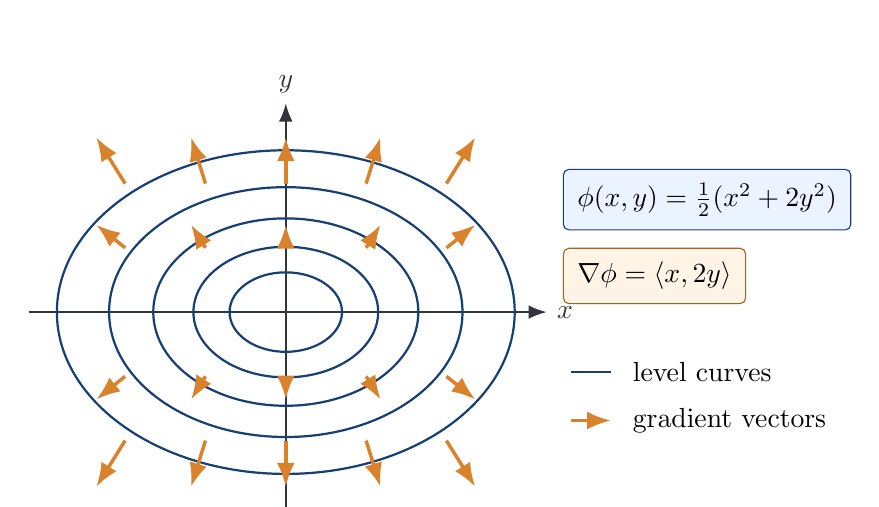
\begin{tikzpicture}[scale=1.02]
  \draw[axisline] (-3.2,0)--(3.25,0) node[right] {$x$};
  \draw[axisline] (0,-2.55)--(0,2.6) node[above] {$y$};
  \foreach \c in {0.7,1.15,1.65,2.2,2.85}{
    \draw[chapterblue!70!black, thick] (0,0) ellipse ({\c} and {0.707*\c});
  }
  \foreach \x in {-2,-1,0,1,2}{
    \foreach \y in {-1.6,-0.8,0.8,1.6}{
      \pgfmathsetmacro{\u}{0.18*\x}
      \pgfmathsetmacro{\v}{0.36*\y}
      \draw[vectororange] (\x,\y) -- +(\u,\v);
    }
  }
  \node[boxnode, anchor=west] at (3.45,1.4) {$\phi(x,y)=\frac12(x^2+2y^2)$};
  \node[orangenode, anchor=west] at (3.45,0.45) {$\grad\phi=\langle x,2y\rangle$};
  \draw[chapterblue!70!black, thick] (3.55,-0.75)--(4.05,-0.75);
  \node[anchor=west] at (4.2,-0.75) {level curves};
  \draw[vectororange] (3.55,-1.35)--(4.05,-1.35);
  \node[anchor=west] at (4.2,-1.35) {gradient vectors};
\end{tikzpicture}
\caption{A gradient field is organized by the level curves of a potential function. The arrows point perpendicular to the level curves.}
\end{figure}

\section{The Fundamental Theorem for Line Integrals}

The one-variable Fundamental Theorem of Calculus says that if $G'(x)=g(x)$, then
\[
\int_a^b g(x)\,dx=G(b)-G(a).
\]
The multivariable version has the same spirit. If a vector field is a gradient field, then its line integral is the change in the potential.

\begin{theorembox}{Fundamental Theorem for Line Integrals}
Let $C$ be a smooth curve from point $A$ to point $B$, and let $f$ be differentiable on a region containing $C$. Then
\[
\int_C \grad f\cdot d\vect r=f(B)-f(A).
\]
Therefore, the integral depends only on the endpoints, not on the path.
\end{theorembox}

\subsection{Why the theorem is true}

Suppose $C$ is parameterized by
\[
\vect r(t)=\langle x(t),y(t)\rangle,\qquad a\le t\le b.
\]
Then
\[
\int_C \grad f\cdot d\vect r
=\int_a^b \grad f(\vect r(t))\cdot \vect r'(t)\,dt.
\]
By the chain rule,
\[
\frac{d}{dt}f(\vect r(t))=\grad f(\vect r(t))\cdot \vect r'(t).
\]
Therefore,
\[
\int_C \grad f\cdot d\vect r
=\int_a^b \frac{d}{dt}f(\vect r(t))\,dt
=f(\vect r(b))-f(\vect r(a)).
\]
The theorem is the chain rule plus the one-variable Fundamental Theorem of Calculus.

\begin{figure}[H]
\centering
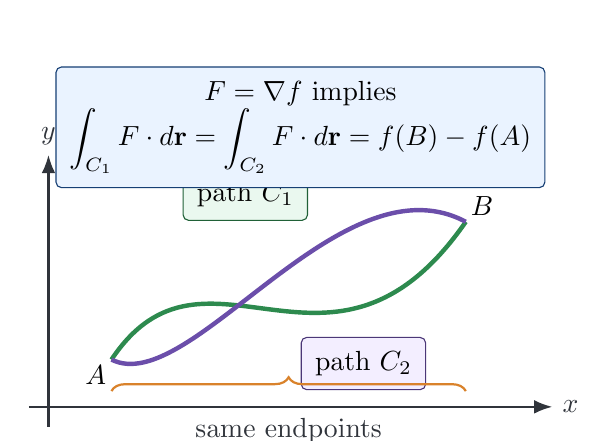
\begin{tikzpicture}[scale=1.0]
  \draw[axisline] (-0.25,0)--(6.4,0) node[right] {$x$};
  \draw[axisline] (0,-0.25)--(0,3.2) node[above] {$y$};
  \coordinate (A) at (0.8,0.6);
  \coordinate (B) at (5.3,2.35);
  \draw[chaptergreen, line width=1.6pt] (A) .. controls (2.0,2.4) and (3.6,-0.1) .. (B);
  \draw[chapterpurple, line width=1.6pt] (A) .. controls (1.8,0.1) and (3.7,3.2) .. (B);
  \fill[startpoint] (A) node[below left] {$A$};
  \fill[endpoint] (B) node[above right] {$B$};
  \node[greennode] at (2.5,2.7) {path $C_1$};
  \node[purplenode] at (4.0,0.55) {path $C_2$};
  \draw[decorate, decoration={brace, amplitude=5pt}, chapterorange, thick] (0.8,0.2)--(5.3,0.2) node[midway,below=6pt, darkgray] {same endpoints};
  \node[boxnode, align=center] at (3.2,3.55) {$F=\grad f$ implies\\$\displaystyle \int_{C_1}F\cdot d\vect r=\int_{C_2}F\cdot d\vect r=f(B)-f(A)$};
\end{tikzpicture}
\caption{For a gradient field, different paths with the same start and end give the same line integral.}
\end{figure}

\begin{examplebox}{Use a potential instead of parameterizing the path}
Let
\[
F(x,y)=\langle 2xy, x^2+3y^2\rangle.
\]
Compute $\int_C F\cdot d\vect r$ for any smooth curve $C$ from $A=(1,0)$ to $B=(2,1)$.

We look for a potential $f$ such that
\[
f_x=2xy,\qquad f_y=x^2+3y^2.
\]
Integrating $f_x=2xy$ with respect to $x$ gives
\[
f(x,y)=x^2y+g(y).
\]
Then $f_y=x^2+g'(y)$. Matching $f_y=x^2+3y^2$ gives $g'(y)=3y^2$ and $g(y)=y^3+C$. One potential is
\[
f(x,y)=x^2y+y^3.
\]
By the Fundamental Theorem for Line Integrals,
\[
\int_C F\cdot d\vect r=f(2,1)-f(1,0)=(4+1)-0=5.
\]
No parameterization of $C$ is needed.
\end{examplebox}

\section{Path independence}

A vector line integral is \textbf{path independent} if any two curves with the same starting point and ending point give the same value. For a conservative field,
\[
\int_C F\cdot d\vect r=f(B)-f(A),
\]
so the integral is path independent. The converse is also true under standard connectedness assumptions: if line integrals of $F$ are path independent on a region, then $F$ is conservative on that region.

\begin{definitionbox}{Equivalent ideas}
For a well-behaved vector field on a suitable region, the following ideas are essentially equivalent:
\begin{enumerate}
  \item $F$ is conservative.
  \item $F=\grad f$ for some potential function $f$.
  \item $\int_C F\cdot d\vect r$ depends only on endpoints.
  \item $\int_C F\cdot d\vect r=0$ for every closed curve $C$.
\end{enumerate}
\end{definitionbox}

\begin{figure}[H]
\centering
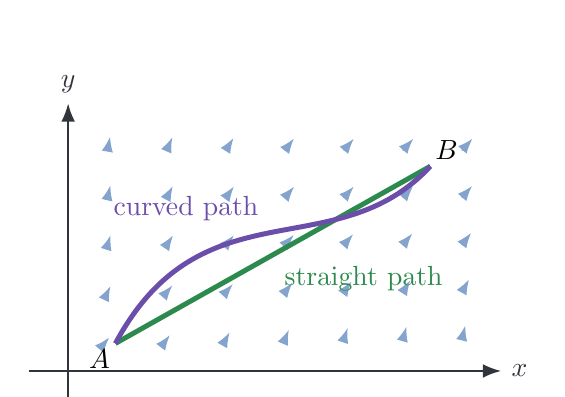
\begin{tikzpicture}[scale=1.0]
  \draw[axisline] (-0.5,0)--(5.5,0) node[right] {$x$};
  \draw[axisline] (0,-0.45)--(0,3.4) node[above] {$y$};
  \foreach \x in {0.5,1.25,...,5.0}{
    \foreach \y in {0.4,1.0,...,3.0}{
      \pgfmathsetmacro{\u}{0.07*(2*\x*\y)}
      \pgfmathsetmacro{\v}{0.045*(\x*\x+3*\y*\y)}
      \pgfmathsetmacro{\len}{sqrt(\u*\u+\v*\v)}
      \draw[chapterblue!55, -Latex, line width=0.55pt] (\x,\y)--+({0.22*\u/(0.25+\len)},{0.22*\v/(0.25+\len)});
    }
  }
  \coordinate (A) at (0.6,0.35);
  \coordinate (B) at (4.6,2.6);
  \draw[chaptergreen, line width=1.8pt] (A)--(B) node[midway,below right] {straight path};
  \draw[chapterpurple, line width=1.8pt] (A) .. controls (1.7,2.4) and (3.4,1.3) .. (B) node[midway,above left] {curved path};
  \fill[startpoint] (A) node[below left] {$A$};
  \fill[endpoint] (B) node[above right] {$B$};
\end{tikzpicture}
\caption{Two different paths from the same start point to the same endpoint. In a conservative field, both paths give the same line integral.}
\end{figure}

\section{How to find a potential function}

Suppose
\[
F(x,y)=\langle P(x,y),Q(x,y)\rangle.
\]
To find a potential function $f$:
\begin{enumerate}
  \item integrate $P=f_x$ with respect to $x$;
  \item include an unknown function of $y$;
  \item differentiate the result with respect to $y$;
  \item compare with $Q=f_y$;
  \item solve for the unknown function.
\end{enumerate}

\begin{figure}[H]
\centering
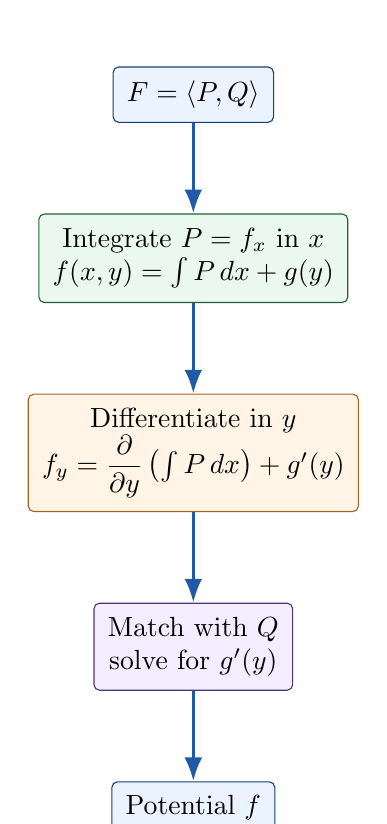
\begin{tikzpicture}[node distance=1.15cm and 1.4cm]
  \node[boxnode] (start) {$F=\langle P,Q\rangle$};
  \node[greennode, below=of start] (intx) {Integrate $P=f_x$ in $x$\\$f(x,y)=\int P\,dx+g(y)$};
  \node[orangenode, below=of intx] (diffy) {Differentiate in $y$\\$f_y=\dfrac{\partial}{\partial y}\left(\int P\,dx\right)+g'(y)$};
  \node[purplenode, below=of diffy] (match) {Match with $Q$\\solve for $g'(y)$};
  \node[boxnode, below=of match] (pot) {Potential $f$};
  \draw[vector] (start)--(intx);
  \draw[vector] (intx)--(diffy);
  \draw[vector] (diffy)--(match);
  \draw[vector] (match)--(pot);
\end{tikzpicture}
\caption{A practical workflow for finding a potential function in the plane.}
\end{figure}

\begin{examplebox}{A conservative field}
Let
\[
F(x,y)=\langle y\cos(xy)+2x,\; x\cos(xy)+4y^3\rangle.
\]
We want $f_x=y\cos(xy)+2x$. Integrating with respect to $x$ gives
\[
f(x,y)=\sin(xy)+x^2+g(y).
\]
Then $f_y=x\cos(xy)+g'(y)$. Matching the second component gives
\[
g'(y)=4y^3,\qquad g(y)=y^4+C.
\]
So one potential is
\[
f(x,y)=\sin(xy)+x^2+y^4.
\]
\end{examplebox}

\section{The component test in the plane}

For a plane vector field $F=\langle P,Q\rangle$, if $F=\grad f$, then
\[
P=f_x,\qquad Q=f_y.
\]
If the second partial derivatives are continuous, then
\[
P_y=f_{xy}=f_{yx}=Q_x.
\]
Therefore, every conservative field satisfies
\[
P_y=Q_x.
\]
On a simply connected region, this condition is also sufficient.

\begin{warningbox}{A necessary condition is not always sufficient}
The equation $P_y=Q_x$ is a local test. It guarantees conservativeness only when the domain has no holes and the field is defined throughout the region. Singularities and holes can create nonzero circulation even when $P_y=Q_x$ away from the singularity.
\end{warningbox}

\begin{examplebox}{Not conservative}
Let $F(x,y)=\langle -y,x\rangle$. Here
\[
P=-y,\qquad Q=x.
\]
Then
\[
P_y=-1,\qquad Q_x=1.
\]
Since $P_y\ne Q_x$, the field is not conservative. This field rotates counterclockwise around the origin. Closed-loop integrals are generally nonzero.
\end{examplebox}

\begin{figure}[H]
\centering
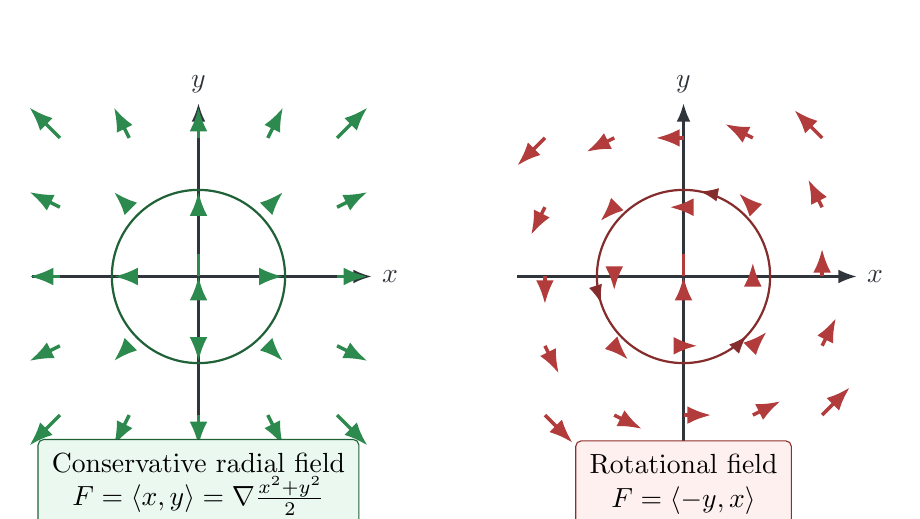
\begin{tikzpicture}[scale=0.88]
  \begin{scope}
    \draw[axisline] (-2.4,0)--(2.5,0) node[right] {$x$};
    \draw[axisline] (0,-2.4)--(0,2.5) node[above] {$y$};
    \foreach \x in {-2,-1,0,1,2}{
      \foreach \y in {-2,-1,0,1,2}{
        \pgfmathsetmacro{\u}{0.22*\x}
        \pgfmathsetmacro{\v}{0.22*\y}
        \draw[vectorgreen] (\x,\y)--+(\u,\v);
      }
    }
    \draw[chaptergreen!70!black, thick] (0,0) circle (1.25);
    \node[greennode] at (0,-3.0) {Conservative radial field\\$F=\langle x,y\rangle=\grad\frac{x^2+y^2}{2}$};
  \end{scope}
  \begin{scope}[xshift=7.0cm]
    \draw[axisline] (-2.4,0)--(2.5,0) node[right] {$x$};
    \draw[axisline] (0,-2.4)--(0,2.5) node[above] {$y$};
    \foreach \x in {-2,-1,0,1,2}{
      \foreach \y in {-2,-1,0,1,2}{
        \pgfmathsetmacro{\u}{-0.20*\y}
        \pgfmathsetmacro{\v}{0.20*\x}
        \draw[vectorred] (\x,\y)--+(\u,\v);
      }
    }
    \draw[chapterred!75!black, thick, postaction={decorate}, decoration={markings, mark=at position 0.22 with {\arrow{Latex}}, mark=at position 0.55 with {\arrow{Latex}}, mark=at position 0.88 with {\arrow{Latex}}}] (0,0) circle (1.25);
    \node[draw=chapterred!80!black, fill=softred, rounded corners=2pt, align=center, inner sep=5pt] at (0,-3.0) {Rotational field\\$F=\langle -y,x\rangle$};
  \end{scope}
\end{tikzpicture}
\caption{A conservative radial field and a rotational field. The rotational field has circulation around closed curves.}
\end{figure}

\section{Closed curves and circulation}

A curve $C$ is \textbf{closed} if its endpoint is the same as its starting point. For a plane field $F=\langle P,Q\rangle$, the line integral around a closed curve is often written
\[
\oint_C F\cdot d\vect r=\oint_C P\,dx+Q\,dy.
\]
This is called the \textbf{circulation} of the vector field around $C$.

If $F$ is conservative, then every closed-loop integral is zero:
\[
\oint_C \grad f\cdot d\vect r=0.
\]
If a closed-loop integral is not zero, then the field cannot be conservative.

\begin{examplebox}{Circulation around a circle}
Let $F(x,y)=\langle -y,x\rangle$, and let $C$ be the circle
\[
\vect r(t)=\langle R\cos t,R\sin t\rangle,\qquad 0\le t\le 2\pi.
\]
Then
\[
d\vect r=\langle -R\sin t,R\cos t\rangle\,dt,
\qquad
F(\vect r(t))=\langle -R\sin t,R\cos t\rangle.
\]
Thus
\[
F(\vect r(t))\cdot \vect r'(t)=R^2\sin^2 t+R^2\cos^2 t=R^2.
\]
Therefore,
\[
\oint_C F\cdot d\vect r=\int_0^{2\pi}R^2\,dt=2\pi R^2.
\]
The circulation is twice the area of the disk.
\end{examplebox}

\section{Green's theorem: circulation form}

Green's theorem converts circulation around a boundary curve into a double integral over the enclosed region. Let $D$ be a plane region with positively oriented boundary curve $C$. Positive orientation means that the region stays on the left as the curve is traversed; for a simple outer boundary, this is counterclockwise orientation.

\begin{theorembox}{Green's Theorem: circulation form}
Let $F=\langle P,Q\rangle$, where $P$ and $Q$ have continuous first partial derivatives on a region containing $D$. If $C$ is the positively oriented boundary of $D$, then
\[
\oint_C P\,dx+Q\,dy
=\iint_D (Q_x-P_y)\,dA.
\]
\end{theorembox}

The quantity $Q_x-P_y$ is the two-dimensional scalar curl of the field. Green's theorem says:

\begin{center}
\Large\bfseries Circulation around the boundary equals total curl inside the region.
\end{center}

\begin{figure}[H]
\centering
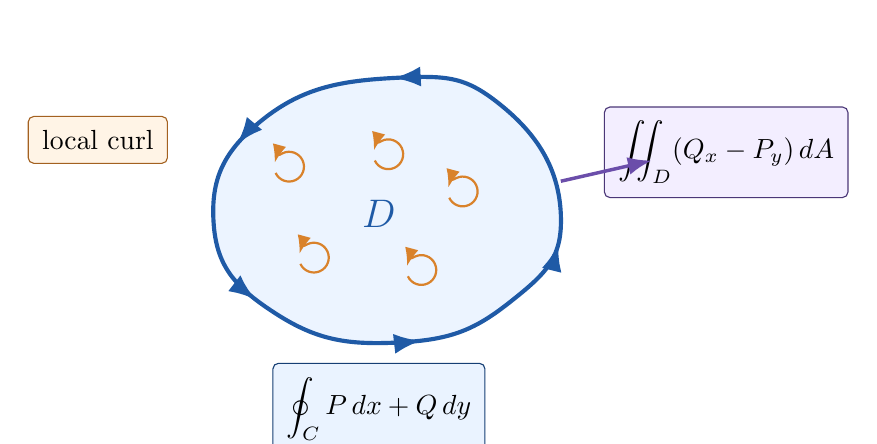
\begin{tikzpicture}[scale=1.05]
  \coordinate (A) at (2.2,0);
  \draw[fill=softblue, opacity=0.9, draw=none]
    plot[smooth cycle, tension=0.8] coordinates {(2.2,0) (1.5,1.3) (0.2,1.65) (-1.4,1.15) (-2.0,-0.1) (-1.25,-1.2) (0.25,-1.55) (1.6,-1.05)};
  \draw[regionboundary]
    plot[smooth cycle, tension=0.8] coordinates {(2.2,0) (1.5,1.3) (0.2,1.65) (-1.4,1.15) (-2.0,-0.1) (-1.25,-1.2) (0.25,-1.55) (1.6,-1.05)};
  \node[font=\Large\bfseries, chapterblue] at (0,0) {$D$};
  \node[boxnode] at (0,-2.35) {$\displaystyle \oint_C P\,dx+Q\,dy$};
  \node[purplenode] at (4.2,0.75) {$\displaystyle \iint_D(Q_x-P_y)\,dA$};
  \draw[vectorpurple] (2.2,0.4)--(3.3,0.65);
  \foreach \x/\y in {-1.1/0.55,0.1/0.7,1.0/0.25,-0.8/-0.55,0.5/-0.7}{
    \draw[chapterorange, thick, -Latex] (\x-0.15,\y-0.05) arc[start angle=205,end angle=525,radius=0.18];
  }
  \node[orangenode] at (-3.4,0.9) {local curl};
\end{tikzpicture}
\caption{Green's theorem relates circulation around a positively oriented boundary to total curl over the enclosed region.}
\end{figure}

\begin{examplebox}{Use Green's theorem on a rectangle}
Let $F(x,y)=\langle -y,x\rangle$. Compute $\oint_C F\cdot d\vect r$ where $C$ is the positively oriented boundary of the rectangle $0\le x\le a$, $0\le y\le b$.

Here $P=-y$ and $Q=x$. Then
\[
Q_x-P_y=1-(-1)=2.
\]
Therefore,
\[
\oint_C -y\,dx+x\,dy=\iint_D 2\,dA=2ab.
\]
The answer is twice the area of the rectangle.
\end{examplebox}

\begin{figure}[H]
\centering
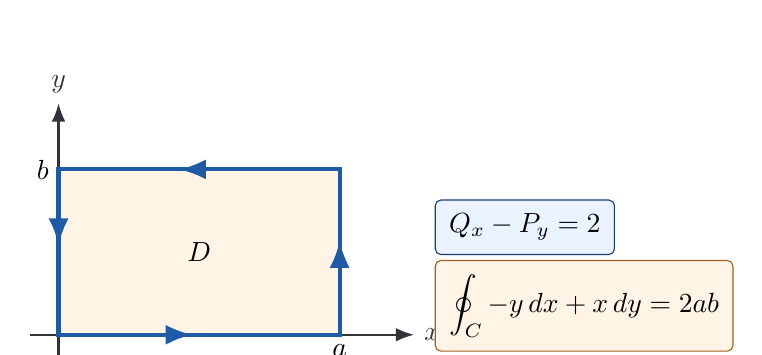
\begin{tikzpicture}[scale=1.05]
  \draw[axisline] (-0.35,0)--(4.3,0) node[right] {$x$};
  \draw[axisline] (0,-0.35)--(0,2.8) node[above] {$y$};
  \fill[softorange] (0,0) rectangle (3.4,2.0);
  \draw[chapterblue, line width=1.5pt, postaction={decorate}, decoration={markings, mark=at position 0.15 with {\arrow{Latex}}, mark=at position 0.42 with {\arrow{Latex}}, mark=at position 0.68 with {\arrow{Latex}}, mark=at position 0.9 with {\arrow{Latex}}}] (0,0)--(3.4,0)--(3.4,2.0)--(0,2.0)--cycle;
  \node[below] at (3.4,0) {$a$};
  \node[left] at (0,2.0) {$b$};
  \node at (1.7,1.0) {$D$};
  \node[boxnode, anchor=west] at (4.55,1.3) {$Q_x-P_y=2$};
  \node[orangenode, anchor=west] at (4.55,0.35) {$\displaystyle \oint_C -y\,dx+x\,dy=2ab$};
\end{tikzpicture}
\caption{For $F=\langle -y,x\rangle$, circulation around a rectangle is twice the area of the rectangle.}
\end{figure}

\section{Area from a line integral}

Green's theorem can be used to compute area. If we choose $P$ and $Q$ so that $Q_x-P_y=1$, then
\[
\operatorname{Area}(D)=\iint_D 1\,dA=\oint_C P\,dx+Q\,dy.
\]
Three common choices are
\[
P=0,\quad Q=x,\qquad \operatorname{Area}(D)=\oint_C x\,dy,
\]
\[
P=-y,\quad Q=0,\qquad \operatorname{Area}(D)=\oint_C -y\,dx,
\]
and the symmetric formula
\[
\operatorname{Area}(D)=\frac12\oint_C x\,dy-y\,dx.
\]

\begin{examplebox}{Area of an ellipse}
Let $C$ be the ellipse
\[
\vect r(t)=\langle a\cos t,b\sin t\rangle,\qquad 0\le t\le 2\pi.
\]
Using $\operatorname{Area}(D)=\frac12\oint_C x\,dy-y\,dx$, we have
\[
x=a\cos t,\quad y=b\sin t,\quad dx=-a\sin t\,dt,\quad dy=b\cos t\,dt.
\]
Thus
\[
x\,dy-y\,dx=ab\cos^2 t\,dt+ab\sin^2 t\,dt=ab\,dt.
\]
Therefore,
\[
\operatorname{Area}(D)=\frac12\int_0^{2\pi}ab\,dt=\pi ab.
\]
\end{examplebox}

\begin{figure}[H]
\centering
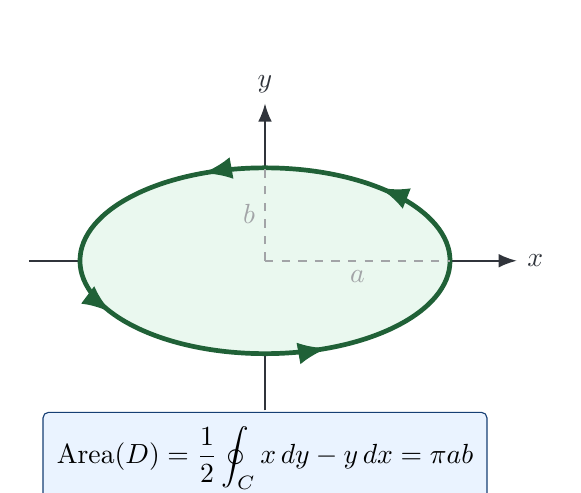
\begin{tikzpicture}[scale=1.0]
  \draw[axisline] (-3,0)--(3.2,0) node[right] {$x$};
  \draw[axisline] (0,-1.9)--(0,2.0) node[above] {$y$};
  \fill[softgreen] (0,0) ellipse (2.35 and 1.18);
  \draw[chaptergreen!70!black, line width=1.7pt, postaction={decorate}, decoration={markings, mark=at position 0.12 with {\arrow{Latex}}, mark=at position 0.32 with {\arrow{Latex}}, mark=at position 0.57 with {\arrow{Latex}}, mark=at position 0.82 with {\arrow{Latex}}}] (0,0) ellipse (2.35 and 1.18);
  \draw[guide] (0,0)--(2.35,0) node[midway,below] {$a$};
  \draw[guide] (0,0)--(0,1.18) node[midway,left] {$b$};
  \node[boxnode] at (0,-2.5) {$\displaystyle \operatorname{Area}(D)=\frac12\oint_C x\,dy-y\,dx=\pi ab$};
\end{tikzpicture}
\caption{Area can be computed from boundary data alone using Green's theorem.}
\end{figure}

\section{Green's theorem: flux form}

Green's theorem also has a flux form. Let $F=\langle P,Q\rangle$. The outward flux across $C$ is
\[
\oint_C F\cdot \vect n\,ds,
\]
where $\vect n$ is the outward unit normal. For a positively oriented plane curve, the outward normal satisfies
\[
\vect n\,ds=\langle dy,-dx\rangle.
\]
Therefore,
\[
F\cdot \vect n\,ds=P\,dy-Q\,dx.
\]
Green's theorem in flux form is
\[
\oint_C F\cdot \vect n\,ds
=\iint_D(P_x+Q_y)\,dA.
\]
The quantity $P_x+Q_y$ is the two-dimensional divergence of $F$.

\begin{tipbox}{Flux interpretation}
Outward flux through the boundary equals total divergence inside the region. This result foreshadows the divergence theorem in three dimensions.
\end{tipbox}

\begin{figure}[H]
\centering
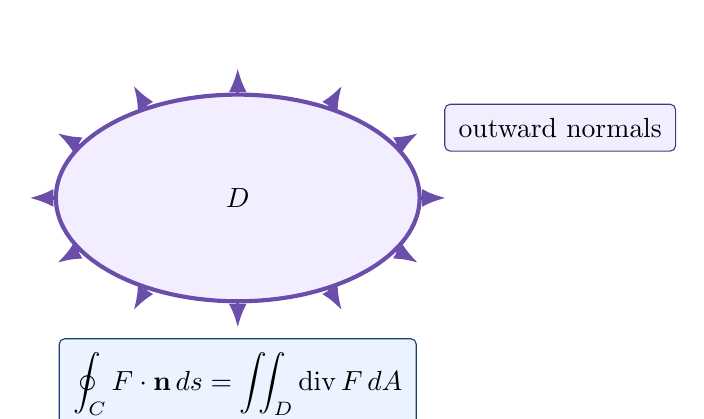
\begin{tikzpicture}[scale=1.05]
  \fill[softpurple] (0,0) ellipse (2.2 and 1.25);
  \draw[chapterpurple, line width=1.5pt] (0,0) ellipse (2.2 and 1.25);
  \foreach \t in {0,30,...,330}{
    \pgfmathsetmacro{\x}{2.2*cos(\t)}
    \pgfmathsetmacro{\y}{1.25*sin(\t)}
    \pgfmathsetmacro{\nx}{0.32*cos(\t)}
    \pgfmathsetmacro{\ny}{0.32*sin(\t)}
    \draw[vectorpurple] (\x,\y)--+(\nx,\ny);
  }
  \node at (0,0) {$D$};
  \node[boxnode] at (0,-2.25) {$\displaystyle \oint_C F\cdot\vect n\,ds=\iint_D\diver F\,dA$};
  \node[purplenode] at (3.9,0.85) {outward normals};
\end{tikzpicture}
\caption{Green's theorem in flux form relates outward flux to total divergence in the region.}
\end{figure}

\begin{examplebox}{Outward flux of a radial field}
Let $F(x,y)=\langle x,y\rangle$. Then
\[
\diver F=P_x+Q_y=1+1=2.
\]
If $C$ bounds a region $D$, then
\[
\oint_C F\cdot \vect n\,ds=\iint_D 2\,dA=2\operatorname{Area}(D).
\]
For a disk of radius $R$, this gives
\[
\oint_C F\cdot \vect n\,ds=2\pi R^2.
\]
\end{examplebox}

\section{Holes, singularities, and why hypotheses matter}

The field
\[
F(x,y)=\left\langle \frac{-y}{x^2+y^2},\frac{x}{x^2+y^2}\right\rangle
\]
is defined everywhere except the origin. Away from the origin, one can check that $P_y=Q_x$. However, the field is not conservative on any region that loops around the origin. On the unit circle $\vect r(t)=\langle \cos t,\sin t\rangle$, we have
\[
F(\vect r(t))=\langle -\sin t,\cos t\rangle=\vect r'(t),
\]
so
\[
\oint_C F\cdot d\vect r=\int_0^{2\pi}1\,dt=2\pi.
\]
The origin is a singularity. The domain has a hole. This example warns that local derivative tests do not always determine global behavior.

\begin{figure}[H]
\centering
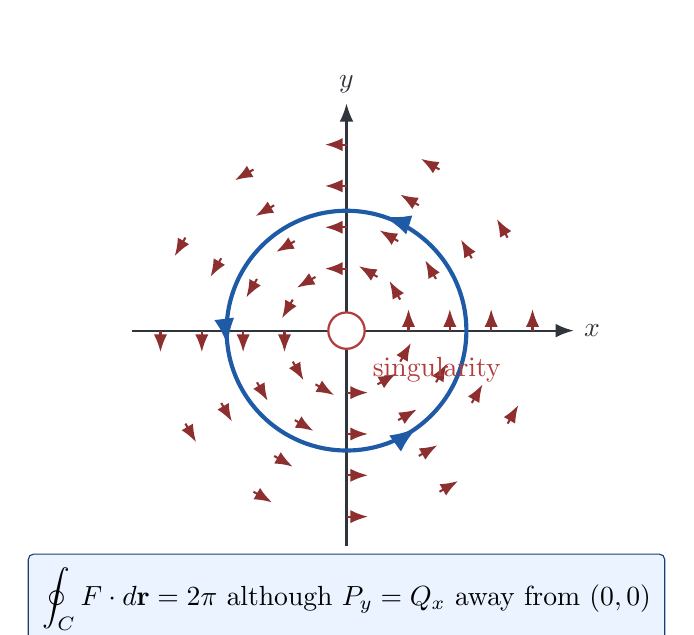
\begin{tikzpicture}[scale=1.05]
  \draw[axisline] (-2.6,0)--(2.75,0) node[right] {$x$};
  \draw[axisline] (0,-2.6)--(0,2.75) node[above] {$y$};
  \foreach \r in {0.75,1.25,1.75,2.25}{
    \foreach \t in {0,30,...,330}{
      \pgfmathsetmacro{\x}{\r*cos(\t)}
      \pgfmathsetmacro{\y}{\r*sin(\t)}
      \pgfmathsetmacro{\u}{-0.26*sin(\t)}
      \pgfmathsetmacro{\v}{0.26*cos(\t)}
      \draw[chapterred!80!black, -Latex, line width=0.75pt] (\x,\y)--+(\u,\v);
    }
  }
  \draw[chapterblue, line width=1.5pt, postaction={decorate}, decoration={markings, mark=at position 0.2 with {\arrow{Latex}}, mark=at position 0.52 with {\arrow{Latex}}, mark=at position 0.85 with {\arrow{Latex}}}] (0,0) circle (1.45);
  \fill[white] (0,0) circle (0.22);
  \draw[chapterred, thick] (0,0) circle (0.22);
  \node[below right, chapterred] at (0.2,-0.2) {singularity};
  \node[boxnode] at (0,-3.25) {$\displaystyle \oint_C F\cdot d\vect r=2\pi$ although $P_y=Q_x$ away from $(0,0)$};
\end{tikzpicture}
\caption{A field with a singularity at the origin. The local curl is zero away from the origin, but the circulation around the origin is nonzero.}
\end{figure}

\section{Numerical curl and discrete Green's theorem intuition}

Green's theorem says that circulation around a boundary measures accumulated curl inside. In computational settings, one often estimates derivatives on a grid. The scalar curl of a plane vector field $F=\langle P,Q\rangle$ is
\[
\curl_{2D}F=Q_x-P_y.
\]
A gradient field has zero scalar curl when second partial derivatives commute. A rotational field has visible nonzero scalar curl.

\begin{figure}[H]
\centering
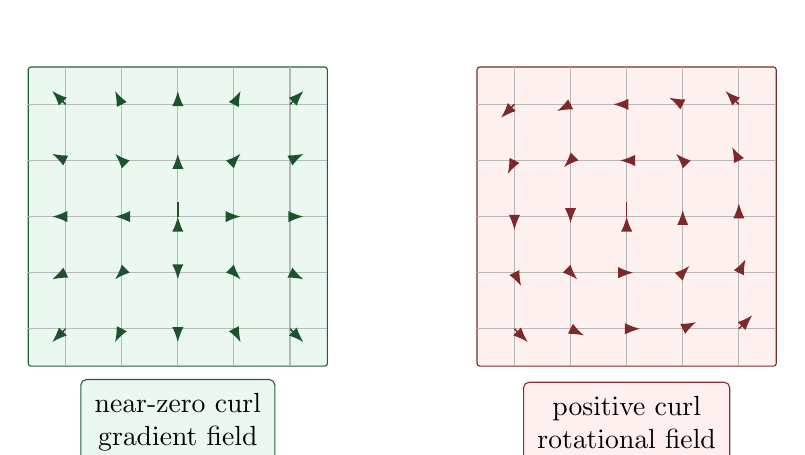
\begin{tikzpicture}[scale=0.95]
  \begin{scope}
    \draw[fill=softgreen, draw=chaptergreen!70!black, rounded corners=1pt] (-2,-2) rectangle (2,2);
    \foreach \x in {-1.5,-0.75,0,0.75,1.5}{\draw[darkgray!35] (\x,-2)--(\x,2);}
    \foreach \y in {-1.5,-0.75,0,0.75,1.5}{\draw[darkgray!35] (-2,\y)--(2,\y);}
    \foreach \x in {-1.5,-0.75,0,0.75,1.5}{
      \foreach \y in {-1.5,-0.75,0,0.75,1.5}{
        \draw[chaptergreen!60!black, -Latex, line width=0.55pt] (\x,\y)--+({0.12*\x},{0.12*\y});
      }
    }
    \node[greennode] at (0,-2.75) {near-zero curl\\gradient field};
  \end{scope}
  \begin{scope}[xshift=6.0cm]
    \draw[fill=softred, draw=chapterred!70!black, rounded corners=1pt] (-2,-2) rectangle (2,2);
    \foreach \x in {-1.5,-0.75,0,0.75,1.5}{\draw[darkgray!35] (\x,-2)--(\x,2);}
    \foreach \y in {-1.5,-0.75,0,0.75,1.5}{\draw[darkgray!35] (-2,\y)--(2,\y);}
    \foreach \x in {-1.5,-0.75,0,0.75,1.5}{
      \foreach \y in {-1.5,-0.75,0,0.75,1.5}{
        \draw[chapterred!70!black, -Latex, line width=0.55pt] (\x,\y)--+({-0.12*\y},{0.12*\x});
      }
    }
    \node[draw=chapterred!80!black, fill=softred, rounded corners=2pt, align=center, inner sep=5pt] at (0,-2.75) {positive curl\\rotational field};
  \end{scope}
\end{tikzpicture}
\caption{Numerical scalar curl can be estimated on a grid. Gradient fields have near-zero curl; rotational fields do not.}
\end{figure}

\section{Modern interpretation: potentials, losses, and dynamics}

In applied mathematics, statistics, data science, and machine learning, a scalar objective function is often the central object:
\[
L(\theta_1,\ldots,\theta_n).
\]
The gradient field $\grad L$ points in the direction of steepest increase, while $-\grad L$ points in the direction of steepest decrease. Gradient descent follows a trajectory determined by a conservative field:
\[
\frac{d\theta}{dt}=-\grad L(\theta).
\]
Along such a path,
\[
\frac{d}{dt}L(\theta(t))=\grad L(\theta(t))\cdot \theta'(t)
=-\norm{\grad L(\theta(t))}^2\le 0.
\]
So a pure gradient flow cannot cycle around a closed loop while strictly decreasing the loss. In contrast, a rotational component can create circulation and oscillation. This distinction matters in dynamical systems, adversarial optimization, non-equilibrium probability flows, and training dynamics for models with coupled parameters.

\begin{figure}[H]
\centering
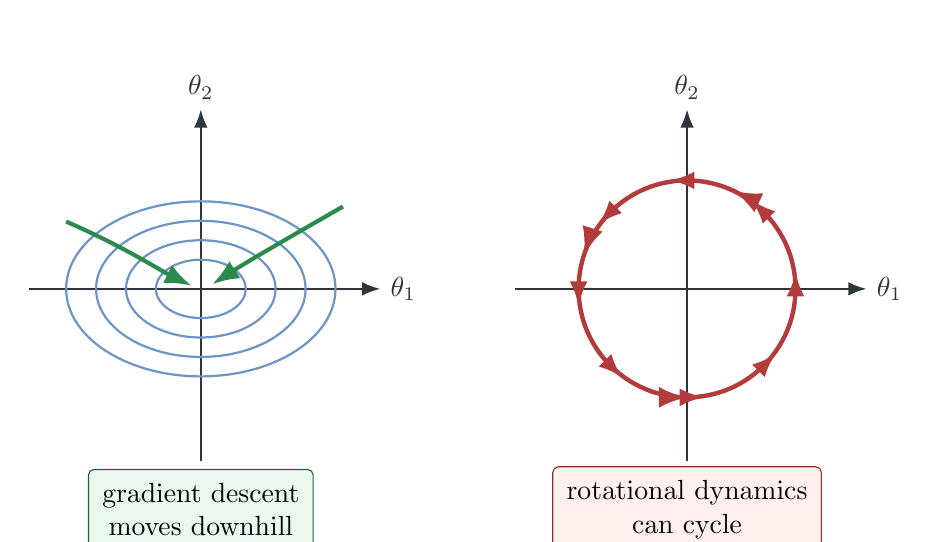
\begin{tikzpicture}[scale=0.95]
  \begin{scope}
    \draw[axisline] (-2.3,0)--(2.4,0) node[right] {$\theta_1$};
    \draw[axisline] (0,-2.3)--(0,2.4) node[above] {$\theta_2$};
    \foreach \r in {0.6,1.0,1.4,1.8}{\draw[chapterblue!65, thick] (0,0) ellipse ({\r} and {0.65*\r});}
    \draw[chaptergreen, line width=1.5pt, -Latex] (1.9,1.1) .. controls (1.2,0.7) and (0.6,0.35) .. (0.15,0.06);
    \draw[chaptergreen, line width=1.5pt, -Latex] (-1.8,0.9) .. controls (-1.0,0.55) and (-0.55,0.25) .. (-0.12,0.04);
    \node[greennode] at (0,-2.95) {gradient descent\\moves downhill};
  \end{scope}
  \begin{scope}[xshift=6.5cm]
    \draw[axisline] (-2.3,0)--(2.4,0) node[right] {$\theta_1$};
    \draw[axisline] (0,-2.3)--(0,2.4) node[above] {$\theta_2$};
    \draw[chapterred, line width=1.6pt, postaction={decorate}, decoration={markings, mark=at position 0.18 with {\arrow{Latex}}, mark=at position 0.45 with {\arrow{Latex}}, mark=at position 0.75 with {\arrow{Latex}}}] (0,0) circle (1.45);
    \foreach \t in {0,45,...,315}{
      \pgfmathsetmacro{\x}{1.45*cos(\t)}
      \pgfmathsetmacro{\y}{1.45*sin(\t)}
      \pgfmathsetmacro{\u}{-0.22*sin(\t)}
      \pgfmathsetmacro{\v}{0.22*cos(\t)}
      \draw[vectorred] (\x,\y)--+(\u,\v);
    }
    \node[draw=chapterred!80!black, fill=softred, rounded corners=2pt, align=center, inner sep=5pt] at (0,-2.95) {rotational dynamics\\can cycle};
  \end{scope}
\end{tikzpicture}
\caption{A pure gradient flow descends a potential landscape, while rotational dynamics can create persistent circulation.}
\end{figure}

\begin{definitionbox}{Conservative versus rotational learning dynamics}
A pure gradient field comes from a scalar objective. A rotational field does not. Many modern algorithms can be viewed as combining gradient-like motion with rotational or momentum-like effects. Green's theorem gives a mathematical language for detecting and measuring circulation in two-dimensional slices of a high-dimensional system.
\end{definitionbox}

\section{Problem-solving guide}

When faced with a line integral of a plane vector field:
\begin{enumerate}
  \item \textbf{Check whether the field is conservative.} Try to find a potential function.
  \item \textbf{If the curve is open and the field is conservative, use endpoints.}
  \item \textbf{If the curve is closed, check Green's theorem.} The boundary integral may become an easier double integral.
  \item \textbf{Check orientation.} Counterclockwise outer boundaries are positive. Reversing orientation changes the sign.
  \item \textbf{Check the domain.} Holes or singularities can invalidate a simple conservative-field conclusion.
  \item \textbf{Choose the easier representation.} Some problems are easier as line integrals; others are easier as double integrals.
\end{enumerate}

\section{Common mistakes}

\begin{warningbox}{Watch for these errors}
\begin{itemize}
  \item Treating $P_y=Q_x$ as sufficient without checking the domain.
  \item Forgetting that Green's theorem requires a closed boundary curve.
  \item Using the wrong orientation and missing a minus sign.
  \item Confusing circulation form with flux form.
  \item Forgetting that a potential function is determined only up to an additive constant.
  \item Applying Green's theorem across a singularity where the field is not defined.
\end{itemize}
\end{warningbox}

\section{Exercises}

\subsection*{Conceptual exercises}
\begin{enumerate}
  \item Explain in your own words what it means for a vector field to be conservative.
  \item Why does a gradient field have zero line integral around every closed curve?
  \item What is the difference between path independence and parameterization independence?
  \item What does Green's theorem say geometrically?
  \item Why does a hole in the domain matter for the conservative-field test?
  \item Explain why the field $F=\langle -y,x\rangle$ should have nonzero circulation around the unit circle.
\end{enumerate}

\subsection*{Computational exercises}
\begin{enumerate}[start=7]
  \item Find a potential function for
  \[
  F(x,y)=\langle 3x^2y+2, x^3+4y\rangle.
  \]
  \item Evaluate $\int_C F\cdot d\vect r$ from $(0,0)$ to $(1,2)$ for the field in Exercise 7.
  \item Determine whether
  \[
  F(x,y)=\langle y^2+e^x,2xy+\cos y\rangle
  \]
  is conservative. If it is, find a potential function.
  \item Compute
  \[
  \oint_C -y\,dx+x\,dy
  \]
  where $C$ is the positively oriented boundary of the triangle with vertices $(0,0)$, $(2,0)$, and $(0,3)$.
  \item Use Green's theorem to compute
  \[
  \oint_C (x^2-y)\,dx+(x+y^2)\,dy
  \]
  where $C$ is the positively oriented boundary of the rectangle $0\le x\le 2$, $0\le y\le 1$.
  \item Use a boundary integral to find the area enclosed by the parametric curve
  \[
  \vect r(t)=\langle 3\cos t,2\sin t\rangle,\qquad 0\le t\le 2\pi.
  \]
  \item Let
  \[
  F(x,y)=\left\langle \frac{-y}{x^2+y^2},\frac{x}{x^2+y^2}\right\rangle.
  \]
  Compute the line integral around the circle of radius $3$ centered at the origin. Explain why the answer does not contradict the local equality $P_y=Q_x$ away from the origin.
\end{enumerate}

\subsection*{Applied and computational exercises}
\begin{enumerate}[start=14]
  \item Let $L(x,y)=x^2+4y^2$. Compute the work done by $\grad L$ along any curve from $(1,1)$ to $(2,0)$.
  \item For the vector field $F=\langle -y,x\rangle$, numerically approximate the circulation around the ellipse $x=2\cos t$, $y=\sin t$. Compare your answer with Green's theorem.
  \item Let $F=\langle P,Q\rangle$ be sampled on a grid. Describe how finite differences could be used to estimate whether $F$ is approximately conservative.
  \item In a learning problem, suppose parameter dynamics show persistent closed-loop motion in a two-dimensional slice of parameter space. Explain why this suggests that the dynamics are not simply pure gradient descent on a scalar loss.
  \item Use Green's theorem to derive the symmetric area formula
  \[
  \operatorname{Area}(D)=\frac12\oint_C x\,dy-y\,dx.
  \]
\end{enumerate}

\section{Chapter summary}

This chapter developed the bridge from line integrals to global vector-calculus theorems.
\begin{itemize}
  \item A vector field is conservative if it is the gradient of a potential function.
  \item Line integrals of conservative fields depend only on endpoints.
  \item The Fundamental Theorem for Line Integrals is the chain rule plus the one-variable Fundamental Theorem of Calculus.
  \item Closed-loop integrals of conservative fields are zero.
  \item In the plane, the condition $P_y=Q_x$ is the local conservative-field test, but the domain matters.
  \item Green's theorem converts circulation around a closed curve into a double integral of scalar curl over the enclosed region.
  \item Green's theorem also has a flux form involving divergence.
  \item Area can be computed from a boundary integral.
  \item Singularities and holes explain why local derivative information may not determine global circulation.
\end{itemize}

In the next chapter, these ideas move from plane regions to surfaces in three-dimensional space. Curl, divergence, surface integrals, and flux are the ingredients needed for Stokes' theorem and the divergence theorem.

\end{document}
